\hypertarget{gtkgridview-and-activate-signal}{%
\section{GtkGridView and activate
signal}\label{gtkgridview-and-activate-signal}}

GtkGridView is similar to GtkListView. It displays a GListModel as a
grid, which is like a square tessellation.

\begin{figure}
\centering
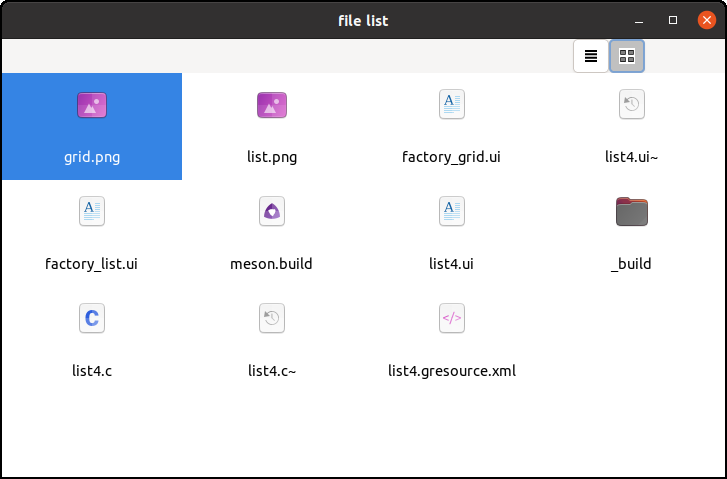
\includegraphics[width=10cm,height=6.6cm]{../image/list4.png}
\caption{Grid}
\end{figure}

This is often seen when you use a file browser like nautilus.

In this section, let's make a very simple file browser
\passthrough{\lstinline!list4!}. It just shows the files in the current
directory. And a user can choose list or grid by clicking on buttons in
the tool bar. Each item in the list or grid has an icon and a filename.
In addition, \passthrough{\lstinline!list4!} provides the way to open
the \passthrough{\lstinline!tfe!} text editor to show a text file. A
user can do that by double clicking on an item or pressing enter key
when an item is selected.

\hypertarget{gtkdirectorylist}{%
\subsection{GtkDirectoryList}\label{gtkdirectorylist}}

GtkDirectoryList implements GListModel and it contains information of
files in a certain directory. The items of the list are GFileInfo
objects.

In the \passthrough{\lstinline!list4!} source files, GtkDirectoryList is
described in a ui file and built by GtkBuilder. The GtkDirectoryList
instance is assigned to the ``model'' property of a GtkSingleSelection
instance. And the GtkSingleSelection instance is assigned to the
``model'' property of a GListView or GGridView instance.

\begin{lstlisting}
GtkListView (model property) => GtkSingleSelection (model property) => GtkDirectoryList
GtkGridView (model property) => GtkSingleSelection (model property) => GtkDirectoryList
\end{lstlisting}

\begin{figure}
\centering
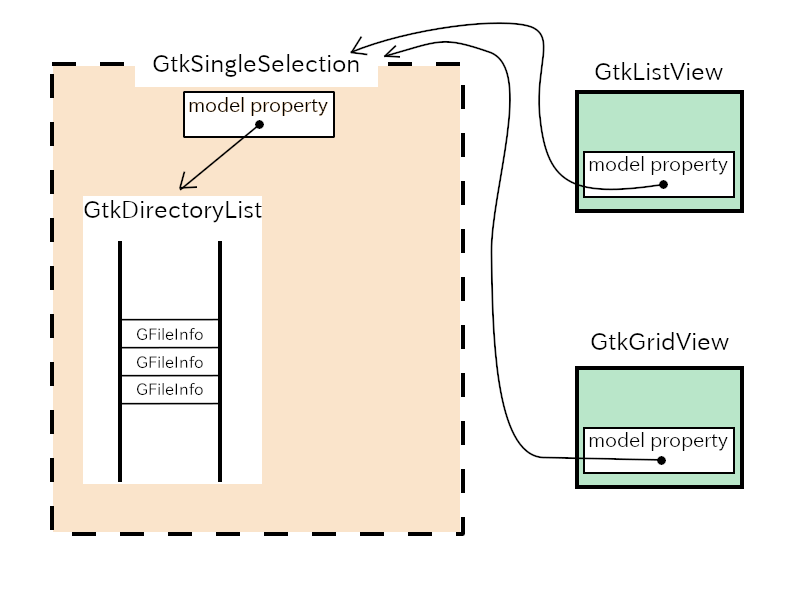
\includegraphics[width=10cm,height=7.5cm]{../image/directorylist.png}
\caption{DirectoryList}
\end{figure}

The following is the part of the ui file
\passthrough{\lstinline!list4.ui!}. It defines GtkListView,
GtkSingleSelection and GtkDirectoryList. It also defines GtkGridView and
GtkSingleSelection.

\begin{lstlisting}[language=XML]
<object class="GtkListView" id="list">
  <property name="model">
    <object class="GtkSingleSelection" id="singleselection">
      <property name="model">
        <object class="GtkDirectoryList" id="directorylist">
          <property name="attributes">standard::name,standard::icon,standard::content-type</property>
        </object>
      </property>
    </object>
  </property>
</object>
<object class="GtkGridView" id="grid">
  <property name="model">singleselection</property>
</object>
\end{lstlisting}

GtkDirectoryList has an ``attributes'' property. It is attributes of
GFileInfo such as ``standard::name'', ``standard::icon'' and
``standard::content-type''.

\begin{itemize}
\tightlist
\item
  standard::name is a filename.
\item
  standard::icon is an icon of the file. It is a GIcon object.
\item
  standard::content-type is a content-type. Content-type is the same as
  mime type for the internet technology. For example, ``text/plain'' is
  a text file, ``text/x-csrc'' is a C source code and so on.
  (``text/x-csrc''is not registered to IANA media types. Such ``x-''
  subtype is not a standard mime type.) Content type is also used by the
  desktop system.
\end{itemize}

GtkGridView has the same structure as GtkListView. But it is enough to
specify its model property to \passthrough{\lstinline!singleselection!}
which is the identification of the GtkSingleSelection. Therefore the
description for GtkGridView is very short.

\hypertarget{ui-file-of-the-window}{%
\subsection{Ui file of the window}\label{ui-file-of-the-window}}

Look at the screenshot of \passthrough{\lstinline!list4!} at the top of
this section. The widgets are built with the following ui file.

\begin{lstlisting}[language=XML, numbers=left]
<?xml version="1.0" encoding="UTF-8"?>
<interface>
  <object class="GtkApplicationWindow" id="win">
    <property name="title">file list</property>
    <property name="default-width">600</property>
    <property name="default-height">400</property>
    <child>
      <object class="GtkBox" id="boxv">
        <property name="orientation">GTK_ORIENTATION_VERTICAL</property>
        <child>
          <object class="GtkBox" id="boxh">
            <property name="orientation">GTK_ORIENTATION_HORIZONTAL</property>
            <child>
              <object class="GtkLabel" id="dmy1">
                <property name="hexpand">TRUE</property>
              </object>
            </child>
            <child>
              <object class="GtkButton" id="btnlist">
                <property name="name">btnlist</property>
                <property name="action-name">win.view</property>
                <property name="action-target">&apos;list&apos;</property>
                <child>
                  <object class="GtkImage">
                    <property name="resource">/com/github/ToshioCP/list4/list.png</property>
                  </object>
                </child>
              </object>
            </child>
            <child>
              <object class="GtkButton" id="btngrid">
                <property name="name">btngrid</property>
                <property name="action-name">win.view</property>
                <property name="action-target">&apos;grid&apos;</property>
                <child>
                  <object class="GtkImage">
                    <property name="resource">/com/github/ToshioCP/list4/grid.png</property>
                  </object>
                </child>
              </object>
            </child>
            <child>
              <object class="GtkLabel" id="dmy2">
                <property name="width-chars">10</property>
              </object>
            </child>
          </object>
        </child>
        <child>
          <object class="GtkScrolledWindow" id="scr">
            <property name="hexpand">TRUE</property>
            <property name="vexpand">TRUE</property>
          </object>
        </child>
      </object>
    </child>
  </object>
  <object class="GtkListView" id="list">
    <property name="model">
      <object class="GtkSingleSelection" id="singleselection">
        <property name="model">
          <object class="GtkDirectoryList" id="directorylist">
            <property name="attributes">standard::name,standard::icon,standard::content-type</property>
          </object>
        </property>
      </object>
    </property>
  </object>
  <object class="GtkGridView" id="grid">
    <property name="model">singleselection</property>
  </object>
</interface>
\end{lstlisting}

The file consists of two parts. The first part begins at the third line
and ends at the 57th line. This part is the widgets from the top level
window to the scrolled window. It also includes two buttons. The second
part begins at the 58th line and ends at the 71st line. This is the part
of GtkListView and GtkGridView. They are described in the previous
section.

\begin{itemize}
\tightlist
\item
  13-17, 42-46: Two labels are dummy labels. They just work as a space
  to put the two buttons at the appropriate position.
\item
  19-41: GtkButton \passthrough{\lstinline!btnlist!} and
  \passthrough{\lstinline!btngrid!}. These two buttons work as selection
  buttons to switch from list to grid and vice versa. These two buttons
  are connected to a stateful action \passthrough{\lstinline!win.view!}.
  This action is stateful and has a parameter. Such action consists of
  prefix, action name and parameter. The prefix of the action is
  \passthrough{\lstinline!win!}, which means the action belongs to the
  top level window. So, a prefix gives the scope of the action. The
  action name is \passthrough{\lstinline!view!}. The parameters are
  \passthrough{\lstinline!list!} or \passthrough{\lstinline!grid!},
  which show the state of the action. A parameter is also called a
  target, because it is a target to which the buttons are clicked on to
  change the action state. We often write the detailed action like
  ``win.view::list'' or ``win.view::grid''.
\item
  21-22: The properties ``action-name'' and ``action-target'' belong to
  GtkActionable interface. GtkButton implements GtkActionable. The
  action name is ``win.view'' and the target is ``list''. Generally, a
  target is GVariant, which can be string, integer, float and so on. You
  need to use GVariant text format to write GVariant value in ui files.
  If the type of the GVariant value is string, then the value with
  GVariant text format is bounded by single quotes or double quotes.
  Because ui file is xml format text, single quote cannot be written
  without escape. Its escape sequence is \&apos;. Therefore, the target
  `list' is written as \&apos;list\&apos;. Because the button is
  connected to the action, ``clicked'' signal handler isn't needed.
\item
  23-27: The child widget of the button is GtkImage. GtkImage has a
  ``resource'' property. It is a GResource and GtkImage reads an image
  data from the resource and sets the image. This resource is built from
  24x24-sized png image data, which is an original icon.
\item
  50-53: GtkScrolledWindow. Its child widget will be GtkListView or
  GtkGridView.
\end{itemize}

The action \passthrough{\lstinline!view!} is created, connected to the
``activate'' signal handler and inserted to the window (action map) as
follows.

\begin{lstlisting}[language=C]
  act_view = g_simple_action_new_stateful ("view", g_variant_type_new("s"), g_variant_new_string ("list"));
  g_signal_connect (act_view, "activate", G_CALLBACK (view_activated), scr); /* scr is the GtkScrolledWindow object */
  g_action_map_add_action (G_ACTION_MAP (win), G_ACTION (act_view));
\end{lstlisting}

The signal handler \passthrough{\lstinline!view\_activated!} will be
explained later.

\hypertarget{factories}{%
\subsection{Factories}\label{factories}}

Each view (GtkListView and GtkGridView) has its own factory because its
items have different structure of widgets. The factories are
GtkBuilderListItemFactory objects. Their ui files are as follows.

factory\_list.ui

\begin{lstlisting}[language=XML, numbers=left]
<?xml version="1.0" encoding="UTF-8"?>
<interface>
  <template class="GtkListItem">
    <property name="child">
      <object class="GtkBox">
        <property name="orientation">GTK_ORIENTATION_HORIZONTAL</property>
        <property name="spacing">20</property>
        <child>
          <object class="GtkImage">
            <binding name="gicon">
              <closure type="GIcon" function="get_icon">
                <lookup name="item">GtkListItem</lookup>
              </closure>
            </binding>
          </object>
        </child>
        <child>
          <object class="GtkLabel">
            <property name="hexpand">TRUE</property>
            <property name="xalign">0</property>
            <binding name="label">
              <closure type="gchararray" function="get_file_name">
                <lookup name="item">GtkListItem</lookup>
              </closure>
            </binding>
          </object>
        </child>
      </object>
    </property>
  </template>
</interface>
\end{lstlisting}

factory\_grid.ui

\begin{lstlisting}[language=XML, numbers=left]
<?xml version="1.0" encoding="UTF-8"?>
<interface>
  <template class="GtkListItem">
    <property name="child">
      <object class="GtkBox">
        <property name="orientation">GTK_ORIENTATION_VERTICAL</property>
        <property name="spacing">20</property>
        <child>
          <object class="GtkImage">
            <property name="icon-size">GTK_ICON_SIZE_LARGE</property>
            <binding name="gicon">
              <closure type="GIcon" function="get_icon">
                <lookup name="item">GtkListItem</lookup>
              </closure>
            </binding>
          </object>
        </child>
        <child>
          <object class="GtkLabel">
            <property name="hexpand">TRUE</property>
            <property name="xalign">0.5</property>
            <binding name="label">
              <closure type="gchararray" function="get_file_name">
                <lookup name="item">GtkListItem</lookup>
              </closure>
            </binding>
          </object>
        </child>
      </object>
    </property>
  </template>
</interface>
\end{lstlisting}

The two files above are almost same. The difference is:

\begin{itemize}
\tightlist
\item
  The orientation of the box
\item
  The icon size
\item
  The position of the text of the label
\end{itemize}

\begin{lstlisting}
$ cd list4; diff factory_list.ui factory_grid.ui
6c6
<         <property name="orientation">GTK_ORIENTATION_HORIZONTAL</property>
---
>         <property name="orientation">GTK_ORIENTATION_VERTICAL</property>
9a10
>             <property name="icon-size">GTK_ICON_SIZE_LARGE</property>
20c21
<             <property name="xalign">0</property>
---
>             <property name="xalign">0.5</property>
\end{lstlisting}

Each view item has two properties, ``gicon'' property of GtkImage and
``label'' property of GtkLabel. Because GFileInfo doesn't have
properties correspond to icon or filename, the factory uses closure tag
to bind ``gicon'' and ``label'' properties to GFileInfo information. A
function \passthrough{\lstinline!get\_icon!} gets GIcon the GFileInfo
object has. And a function \passthrough{\lstinline!get\_file\_name!}
gets a filename the GFileInfo object has.

\begin{lstlisting}[language=C, numbers=left]
GIcon *
get_icon (GtkListItem *item, GFileInfo *info) {
  GIcon *icon;

  if (! G_IS_FILE_INFO (info))
    return NULL;
  else {
    icon = g_file_info_get_icon (info);
    g_object_ref (icon);
    return icon;
  }
}

char *
get_file_name (GtkListItem *item, GFileInfo *info) {
  if (! G_IS_FILE_INFO (info))
    return NULL;
  else
    return g_strdup (g_file_info_get_name (info));
}
\end{lstlisting}

One important thing is view items own the instance or string. It is
achieved by \passthrough{\lstinline!g\_object\_ref!} to increase the
reference count by one, or \passthrough{\lstinline!strdup!} to create a
copy of the string. The object or string will be automatically freed in
unbinding process when the view item is recycled.

\hypertarget{an-activate-signal-handler-of-the-action}{%
\subsection{An activate signal handler of the
action}\label{an-activate-signal-handler-of-the-action}}

An activate signal handler \passthrough{\lstinline!view\_activate!}
switches the view. It does two things.

\begin{itemize}
\tightlist
\item
  Changes the child widget of GtkScrolledWindow.
\item
  Changes the CSS of buttons to show the current state.
\end{itemize}

\begin{lstlisting}[language=C, numbers=left]
static void
view_activated(GSimpleAction *action, GVariant *parameter, gpointer user_data) {
  GtkScrolledWindow *scr = GTK_SCROLLED_WINDOW (user_data);
  const char *view = g_variant_get_string (parameter, NULL);
  const char *other;
  char *css;

  if (strcmp (view, "list") == 0) {
    other = "grid";
    gtk_scrolled_window_set_child (scr, list);
  }else {
    other = "list";
    gtk_scrolled_window_set_child (scr, grid);
  }
  css = g_strdup_printf ("button#btn%s {background: silver;} button#btn%s {background: white;}", view, other);
  gtk_css_provider_load_from_data (provider, css, -1);
  g_free (css);
  g_action_change_state (G_ACTION (action), parameter);
}
\end{lstlisting}

The second parameter of this handler is the target of the clicked
button. Its type is GVariant.

\begin{itemize}
\tightlist
\item
  If \passthrough{\lstinline!btnlist!} has been clicked, then
  \passthrough{\lstinline!parameter!} is a GVariant of the string
  ``list''.
\item
  If \passthrough{\lstinline!btngrid!} has been clicked, then
  \passthrough{\lstinline!parameter!} is a GVariant of the string
  ``grid''.
\end{itemize}

The third parameter \passthrough{\lstinline!user\_data!} points
GtkScrolledWindow, which is set in the
\passthrough{\lstinline!g\_signal\_connect!} function.

\begin{itemize}
\tightlist
\item
  4: \passthrough{\lstinline!g\_variant\_get\_string!} gets the string
  from the GVariant variable.
\item
  8-14: Sets the child of \passthrough{\lstinline!scr!}. The function
  \passthrough{\lstinline!gtk\_scrolled\_window\_set\_child!} decreases
  the reference count of the old child by one. And it increases the
  reference count of the new child by one.
\item
  15-17: Sets the CSS of the buttons. The background of the clicked
  button will be silver color and the other button will be white.
\item
  18: Changes the state of the action.
\end{itemize}

\hypertarget{activate-signal-of-gtklistview-and-gtkgridview}{%
\subsection{Activate signal of GtkListView and
GtkGridView}\label{activate-signal-of-gtklistview-and-gtkgridview}}

Views (GtkListView and GtkGridView) have an ``activate'' signal. It is
emitted when an item in the view is double clicked or the enter key is
pressed. You can do anything you like by connecting the ``activate''
signal to the handler.

The example \passthrough{\lstinline!list4!} launches
\passthrough{\lstinline!tfe!} text file editor if the item of the list
is a text file.

\begin{lstlisting}[language=C]
static void
list_activate (GtkListView *list, int position, gpointer user_data) {
  GFileInfo *info = G_FILE_INFO (g_list_model_get_item (G_LIST_MODEL (gtk_list_view_get_model (list)), position));
  launch_tfe_with_file (info);
}

static void
grid_activate (GtkGridView *grid, int position, gpointer user_data) {
  GFileInfo *info = G_FILE_INFO (g_list_model_get_item (G_LIST_MODEL (gtk_grid_view_get_model (grid)), position));
  launch_tfe_with_file (info);
}

... ...
... ...

  g_signal_connect (GTK_LIST_VIEW (list), "activate", G_CALLBACK (list_activate), NULL);
  g_signal_connect (GTK_GRID_VIEW (grid), "activate", G_CALLBACK (grid_activate), NULL);
\end{lstlisting}

The second parameter of the handlers is the position of the item
(GFileInfo) of the GListModel. So you can get the item with
\passthrough{\lstinline!g\_list\_model\_get\_item!} function.

\hypertarget{content-type-and-launching-an-application}{%
\subsection{Content type and launching an
application}\label{content-type-and-launching-an-application}}

The function \passthrough{\lstinline!launch\_tfe\_with\_file!} gets a
file from the GFileInfo instance. If the file is a text file, it
launches \passthrough{\lstinline!tfe!} with the file.

GFileInfo has information about file type. The file type is like
``text/plain'', ``text/x-csrc'' and so on. It is called content type.
Content type can be got with
\passthrough{\lstinline!g\_file\_info\_get\_content\_type!} function.

\begin{lstlisting}[language=C, numbers=left]
static void
launch_tfe_with_file (GFileInfo *info) {
  GError *err = NULL;
  GFile *file;
  GList *files = NULL;
  const char *content_type;
  const char *text_type = "text/";
  GAppInfo *appinfo;
  int i;

  if (! info)
    return;
  content_type = g_file_info_get_content_type (info);
g_print ("%s\n", content_type);  /* This line can be commented out if unnecessary */
  if (! content_type)
    return;
  for (i=0;i<5;++i) {
    if (content_type[i] != text_type[i])
      return;
  }
  appinfo = g_app_info_create_from_commandline ("tfe", "tfe", G_APP_INFO_CREATE_NONE, &err);
  if (err) {
    g_printerr ("%s\n", err->message);
    g_error_free (err);
    return;
  }
  err = NULL;
  file = g_file_new_for_path (g_file_info_get_name (info));
  files = g_list_append (files, file);
  if (! (g_app_info_launch (appinfo, files, NULL, &err))) {
    g_printerr ("%s\n", err->message);
    g_error_free (err);
  }
  g_list_free_full (files, g_object_unref);
  g_object_unref (appinfo);
}
\end{lstlisting}

\begin{itemize}
\tightlist
\item
  13: Gets the content type of the file from GFileInfo.
\item
  14: Prints the content type. This is only useful to know a content
  type of a file. You can delete it if unnecessary.
\item
  17-20: If the content type doesn't begin with ``text/'', then it
  returns.
\item
  21: Creates GAppInfo object of \passthrough{\lstinline!tfe!}
  application. GAppInfo is an interface and the variable
  \passthrough{\lstinline!appinfo!} points a GDesktopAppInfo instance.
  GAppInfo is a collection of information of an application.
\item
  30: Launches the application (\passthrough{\lstinline!tfe!}) with an
  argument \passthrough{\lstinline!file!}.
  \passthrough{\lstinline!g\_app\_info\_launch!} has four parameters.
  The first parameter is GAppInfo object. The second parameter is a list
  of GFile objects. In this function, only one GFile instance is given
  to \passthrough{\lstinline!tfe!}, but you can give more arguments. The
  third parameter is GAppLaunchContext, but this program gives NULL
  instead. The last parameter is the pointer to the pointer to a GError.
\item
  34: \passthrough{\lstinline!g\_list\_free\_full!} frees the memories
  used by the list and items.
\end{itemize}

If your distribution supports Gtk4, using
\passthrough{\lstinline!g\_app\_info\_launch\_default\_for\_uri!} is
convenient. The function automatically determines the default
application from the file and launches it. For example, if the file is
text, then it launches gedit with the file. Such functionality comes
from desktop.

\hypertarget{compilation-and-execution}{%
\subsection{Compilation and execution}\label{compilation-and-execution}}

The source files are located in src/list4 directory. To compile and
execute list4, type as follows.

\begin{lstlisting}
$ cd list4 # or cd src/list4. It depends your current directory.
$ meson _build
$ ninja -C _build
$ _build/list4
\end{lstlisting}

Then a file list appears as a list style. Click on a button on the tool
bar so that you can change the style to grid or back to list. Double
click ``list4.c'' item, then \passthrough{\lstinline!tfe!} text editor
runs with the argument ``list4.c''. The following is the screenshot.

\begin{figure}
\centering
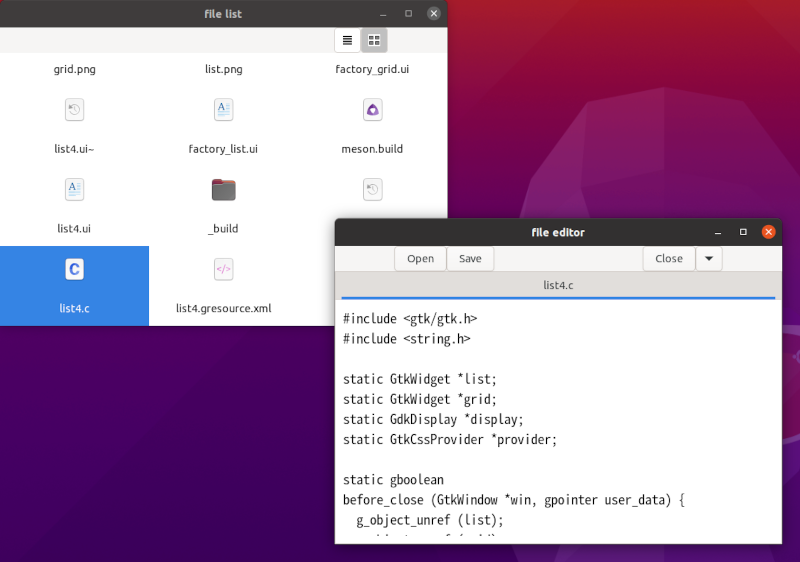
\includegraphics[width=8cm,height=5.62cm]{../image/screenshot_list4.png}
\caption{Screenshot}
\end{figure}

\hypertarget{gbytes-property-of-gtkbuilderlistitemfactory}{%
\subsection{``gbytes'' property of
GtkBuilderListItemFactory}\label{gbytes-property-of-gtkbuilderlistitemfactory}}

GtkBuilderListItemFactory has ``gbytes'' property. The property contains
a byte sequence of ui data. If you use this property, you can put the
contents of \passthrough{\lstinline!factory\_list.ui!} and
\passthrough{\lstinline!factory\_grid.ui!}into
\passthrough{\lstinline!list4.ui!}. The following shows a part of the
new ui file (\passthrough{\lstinline!list5.ui!}).

\begin{lstlisting}[language=XML]
  <object class="GtkListView" id="list">
    <property name="model">
      <object class="GtkSingleSelection" id="singleselection">
        <property name="model">
          <object class="GtkDirectoryList" id="directorylist">
            <property name="attributes">standard::name,standard::icon,standard::content-type</property>
          </object>
        </property>
      </object>
    </property>
    <property name="factory">
      <object class="GtkBuilderListItemFactory">
        <property name="bytes"><![CDATA[
<?xml version="1.0" encoding="UTF-8"?>
<interface>
  <template class="GtkListItem">
    <property name="child">
      <object class="GtkBox">
        <property name="orientation">GTK_ORIENTATION_HORIZONTAL</property>
        <property name="spacing">20</property>
        <child>
          <object class="GtkImage">
            <binding name="gicon">
              <closure type="GIcon" function="get_icon">
                <lookup name="item">GtkListItem</lookup>
              </closure>
            </binding>
          </object>
        </child>
        <child>
          <object class="GtkLabel">
            <property name="hexpand">TRUE</property>
            <property name="xalign">0</property>
            <binding name="label">
              <closure type="gchararray" function="get_file_name">
                <lookup name="item">GtkListItem</lookup>
              </closure>
            </binding>
          </object>
        </child>
      </object>
    </property>
  </template>
</interface>
        ]]></property>
      </object>
    </property>
  </object>
\end{lstlisting}

CDATA section begins with ``\textless{[}CDATA{[}" and ends with
"{]}{]}\textgreater{}''. The contents of CDATA section is recognized as
a string. Any character, even if it is a key syntax marker such as
`\textless{}' or `\textgreater{}', is recognized literally. Therefore,
the text between ``\textless{[}CDATA{[}" and "{]}{]}\textgreater{}'' is
inserted to ``bytes'' property as it is.

This method decreases the number of ui files. But, the new ui file is a
bit complicated especially for the beginners. If you feel some
difficulty, it is better for you to separate the ui file.

A directory src/list5 includes the ui file above.
